\documentclass[12pt]{article}
\usepackage[margin=2.5cm]{geometry}
\usepackage[utf8]{inputenc}
\usepackage[version=4]{mhchem}
\usepackage{graphicx}
\usepackage{placeins}
\usepackage{chemfig}
\usepackage{epstopdf}

\title{Chemistry2 TP3}
\author{Louis-Hendrik Barboutie}
\date{March 2022}

\begin{document}

\begin{titlepage}
    \begin{center}
        \vspace*{1cm}
        \Huge
        \textbf{Solvolysis \ce{S_N 1} of alkyl halides}
        
        \vspace{0.5cm}
        \LARGE
        Chemistry 2 - TP 3
        
        \vspace{1.5cm}
        \textbf{Louis-Hendrik Barboutie}
        
        \vfill
        

        
\includegraphics[width=0.4\textwidth]{logo_uni.jpg}
        
        \Large
        23rd March 2022
    \end{center}
\end{titlepage}

\section{Abstract}
The main goal of this experiment is to determine the rate law of the solvolysis $\text{S}_\text{N}$1 reaction of t-butyl chloride. This is achieved by running a fast clock reaction along the solvolysis reaction to determine its speed. The experiment is repeated for different concentrations of t-BuCl at room temperature, then at 0°C. The rate law constants have been determined to be $k = (2.2\pm1.3)\cdot 10^{-2}$ and $n \approx 2$ and the activation energy has been calculated to be $E_a \approx 1.1 \cdot 10^{-22}$ J. 

\section{Introduction}
We are interested in studying the speed of the solvolysis reaction of t-butyl chloride in water. The solvolysis reaction of t-butyl chloride is: \begin{equation}
    \ce{(H3C)3C-Cl + H2O -> (H3C)3C-OH + H+ + Cl-}
\end{equation} It is a substitution reaction, where one group of the molecule gets replaced by another. In this case, \ce{Cl-} is the leaving group, and \ce{OH-} takes its place. Since the resulting molecule is an alcohol, we need to use a mixture of solvents, because alcohols aren't very miscible with water, but soluble in acetone, which is itself soluble in water. This is why we use a mixture of water-acetone solvent. 

\noindent The individual steps of the reaction are:

\begin{center}
\schemestart
    \chemfig{C([3]-H_3C)([:190]<:H_3C)([5]<H_3C)-[@{db}]@{a1}Cl}
    \+
    \chemfig{\charge{135=\:,225=\:}{O}([1]-H)([-1]-H)}
    \arrow{->}
    \chemfig{@{ce}C^+([3]-H_3C)([:190]<:H_3C)([5]<H_3C)}
    \+
    \chemfig{@{dbe}\charge{135=\:,225=\:}{O}([1]-H)(-[@{sb}::-45]@{sh}{H})}
    \+
    \chemfig{@{ccl}\charge{30=$^-$}{Cl}}
\schemestop
\chemmove{\draw[shorten <= 2pt, shorten >= 2pt](db)..controls +(90:7mm) and +(90:7mm)..(a1);}
\chemmove{\draw[shorten <= 5pt, shorten >= 2pt](dbe)..controls +(135:8mm) and +(45:8mm)..(ce);\draw[shorten <= 2pt, shorten >= 2pt](sb)..controls +(45:3mm) and +(0:5mm)..(dbe);\draw[shorten <= 2pt, shorten >= 2pt](ccl)..controls +(-90:8mm) and +(0:8mm)..(sh);}
\end{center}

\noindent Then the final result is: \medskip
    
\begin{center}
\schemestart
    \chemfig{H-Cl}
    \+
    \chemfig{C(-[3]H_3C)(<:[:190]H_3C)(<[5]H_3C)-\charge{[circle]90=\|,-90=\|}{O}-H}
\schemestop
\end{center}

\noindent The rate determining step of this reaction, i.e. the slowest step to take place is the separation of the leaving group from the molecule. In this case it is the separation of \ce{Cl-} from \ce{(H3C)3C+}. We can use the formation of hydrochloric acid to our advantage to time the reaction. By adding sodium hydroxide, reaction (2) takes place.

\begin{equation}
    \ce{H+ + Cl- + NaOH -> 2H2O +NaCl} 
\end{equation}

\noindent It is called the clock reaction and happens very fast because sodium hydroxide is a strong base. The reactants are an acid and a base, whereas the products are pH-neutral. With a color indicator, eg. bromothymol, the end of this reaction can be visualized. If much more hydrochloric acid forms than sodium hydroxide is added, then the solution will be basic before the reaction, and once all the sodium hydroxide is consumed acidic because of the remaining hydrochloric acid. Bromothymol blue is blue in basic environments and yellow in acidic environments, and therefore is an excellent choice for this reaction.

\noindent The rate of the reaction, i.e. how fast it occurs can be described by the relationship: \begin{equation}\nu_0 = k \cdot [reactant]^n \label{eq:rate}\end{equation} Note that since water is the second reactant, and is in surplus, it is not taken into account. We will determine k and n with this experiment. An initial estimate for n is n = 1. 

\section{Experiment}

\subsection{Chemicals used}
For the experiment, the chemicals required are:
\begin{enumerate}
    \item Water (\ce{H2O})
    \item Sodium hydroxide (\ce{NaOH})
    \item Acetone (\ce{C3H6O}) \cite{Acetone}
    \item Bromothymol (\ce{C27H28Br2O5S}) \cite{Bromothymol}
    \item T-butyl chloride (\ce{C4H9Cl}) \cite{T-Butyl Chloride}
\end{enumerate}

\subsection{Safety equipment}

The chemicals used are corrosive, highly flammable and irritating, the chemist is therefore advised to wear safety goggles, a lab coat and nitril gloves at all times.

\subsection{Setup}

The setup for this experiment is depicted in figure~(\ref{fig:setup})
\begin{figure}[!ht]
    \centering
    \resizebox{0.45\textwidth}{!}{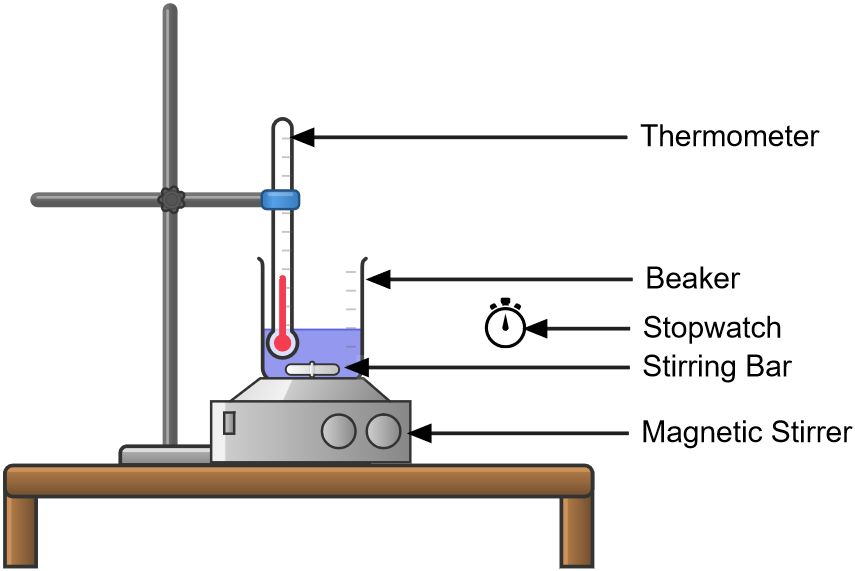
\includegraphics{Setup.jpg}}
    \caption{Setup of the experiment}
    \label{fig:setup}
\end{figure}
\FloatBarrier

\clearpage
\noindent Other containers and measurement devices (not shown) are: \begin{itemize}
    \item 100 mL beakers 
    \item 5 mL, 10 mL, 25 mL pipettes
\end{itemize}

\subsection{Measurement of the reaction speed at 25°C}

\subsubsection{Preparation of the solutions}

In order to obtain insight on the reaction speed, four solutions, of total volume 26 mL, with different concentrations of t-butyl chloride and acetone are prepared (see table (\ref{tab:SolPrep})). Note that the provided t-BuCl solution has concentration of 0.184 M and the NaOH solution has concentration of 0.006 M. The NaOH and the t-butyl chloride are sampled with a 5 mL pipette, the water with a 10 mL pipette and the acetone with a 25 mL pipette. The bromothymol is added to the solution with a pasteur pipette.
    
\begin{table}[h!]
    \centering
    \resizebox{\textwidth}{!}{\begin{tabular}{c|c|c|c|c|c}
        Number & $V_{\ce{NaOH}}$ (mL) & $V_{\ce{H2O}}$ (mL) & $V_{\ce{C3H6O}}$ (mL) & Bromothymol (drops) & $V_{\ce{t-BuCl}}$ (mL) \\ \hline
        1 & 3.0 & 10.0 & 12.0 & 5 & 1.0 \\ 
        2 & 3.0 & 10.0 & 11.0 & 5 & 2.0 \\ 
        3 & 3.0 & 10.0 & 10.0 & 5 & 3.0 \\ 
        4 & 3.0 & 10.0 &  9.0 & 5 & 4.0 \\
        5 & 3.0 & 10.0 &  9.5 & 5 & 3.5 
    \end{tabular}}
    \caption{Solution preparation}
    \label{tab:SolPrep}
\end{table}

\subsubsection{Measurement}
Once the t-BuCl is indroduced in the beaker, the reaction begins and we start the stopwatch. When the solution changes colour due to the bromothymol inside, we stop the stopwatch, and record the elapsed time.

\subsection{Measurement of the reaction speed at 0°C}
The same experiment is repeated with solution number 4 at 273 K to see if temperature affects the reaction speed. The beaker is therefore plunged in an ice bath until the temperature sinks to 273 K, and then the reaction is started and the time recorded. 

\subsection{Error Calculation}

\subsubsection{Instrumental error}

The error of the 5 mL pipette is $\pm$ 0.03 mL, of the 10 mL pipette it is $\pm 0.05$ mL and of the 25 mL pipette it is $\pm 0.1$ mL

\subsubsection{Operator error}

Since we have no precise way of timing the reaction, and the transfer of t-butyl chloride into the solution is not instantaneous, a generous 5 s of error is added to the elapsed time measurement. Due to the volatile nature and improper storage of t-BuCl and Acetone, their concentrations may have changed during the experiment, adding additional error.   

\subsubsection{Formulae}

For additive (or substractive) formulae, of the form \[ X = A \pm B\] the error is : \[\Delta X = \Delta A + \Delta B\]
For multiplicative (or divisive) formulae of the form \[X = A \cdot  B^{\pm 1}\] the error is: \[  \Delta X = X\sqrt{\left(\frac{\Delta A}{A}\right)^2+\left(\frac{\Delta B}{B}\right)^2} \]
For functional relationships: $Y=f(X)$ the error is: \[ \frac{\Delta Y}{Y} = \sqrt{\left|\frac{\partial f}{\partial X}\right|^2(\Delta X)^2} \]

\section{Results and discussion}

\subsection{Measurement of the reaction speed at 25°C}

\begin{table}[!ht]
    \centering
    \begin{tabular}{c|c|c}
        Solution & $\Delta$ t & Temperature ($^{\circ}$C) \\ \hline
        1 & $>$ 25' & 23 \\
        4 & $>$ 5' & 24
    \end{tabular}
    \caption{Reaction times with the first provided solution of t-butyl chloride}
    \label{tab:results1}
\end{table}

\noindent After 25 minutes and no change in colour, the first the experiment was stopped, as it shouldn't take such a long time. In order to identify the source of the problem, the experiment was repeated with the solution with the highest concentration. It should have been a fast reaction, no longer than three minutes. After 5 minutes it was also interrupted, as no colour change had happened. Both these experiments give evidence that the concentration of the t-butyl chloride was not the same as on the label. 

\noindent The experiment was then repeated with a different t-butyl chloride solution, as seen in table~(\ref{tab:results2}). This time, it was successful, and the colour change could be observed.

\begin{table}[!ht]
    \centering
    \begin{tabular}{c|c|c}
        Solution & $\Delta$ t  & Temperature ($^{\circ}$C) \\ \hline
        2 & 2'52'' $\pm$ 5'' & 26 \\
        3 & 1'48'' $\pm$ 5'' & 25 \\
        4 & 1'02'' $\pm$ 5'' & 26 \\
        5 & 1'56'' $\pm$ 5'' & 25
    \end{tabular}
    \caption{Reaction times with the second provided solution of t-butyl chloride}
    \label{tab:results2}
\end{table}
\FloatBarrier

\noindent During both experiments, no change in temperature besides fluctuations in the room temperature could be observed. We conclude, that the speed of the reaction does not have an influence on the temperature of the solution.

\noindent The graph seen in figure (2) shows the results obtained when measuring the time.

\begin{figure}[!ht]
    \centering
    \resizebox{0.7\textwidth}{!}{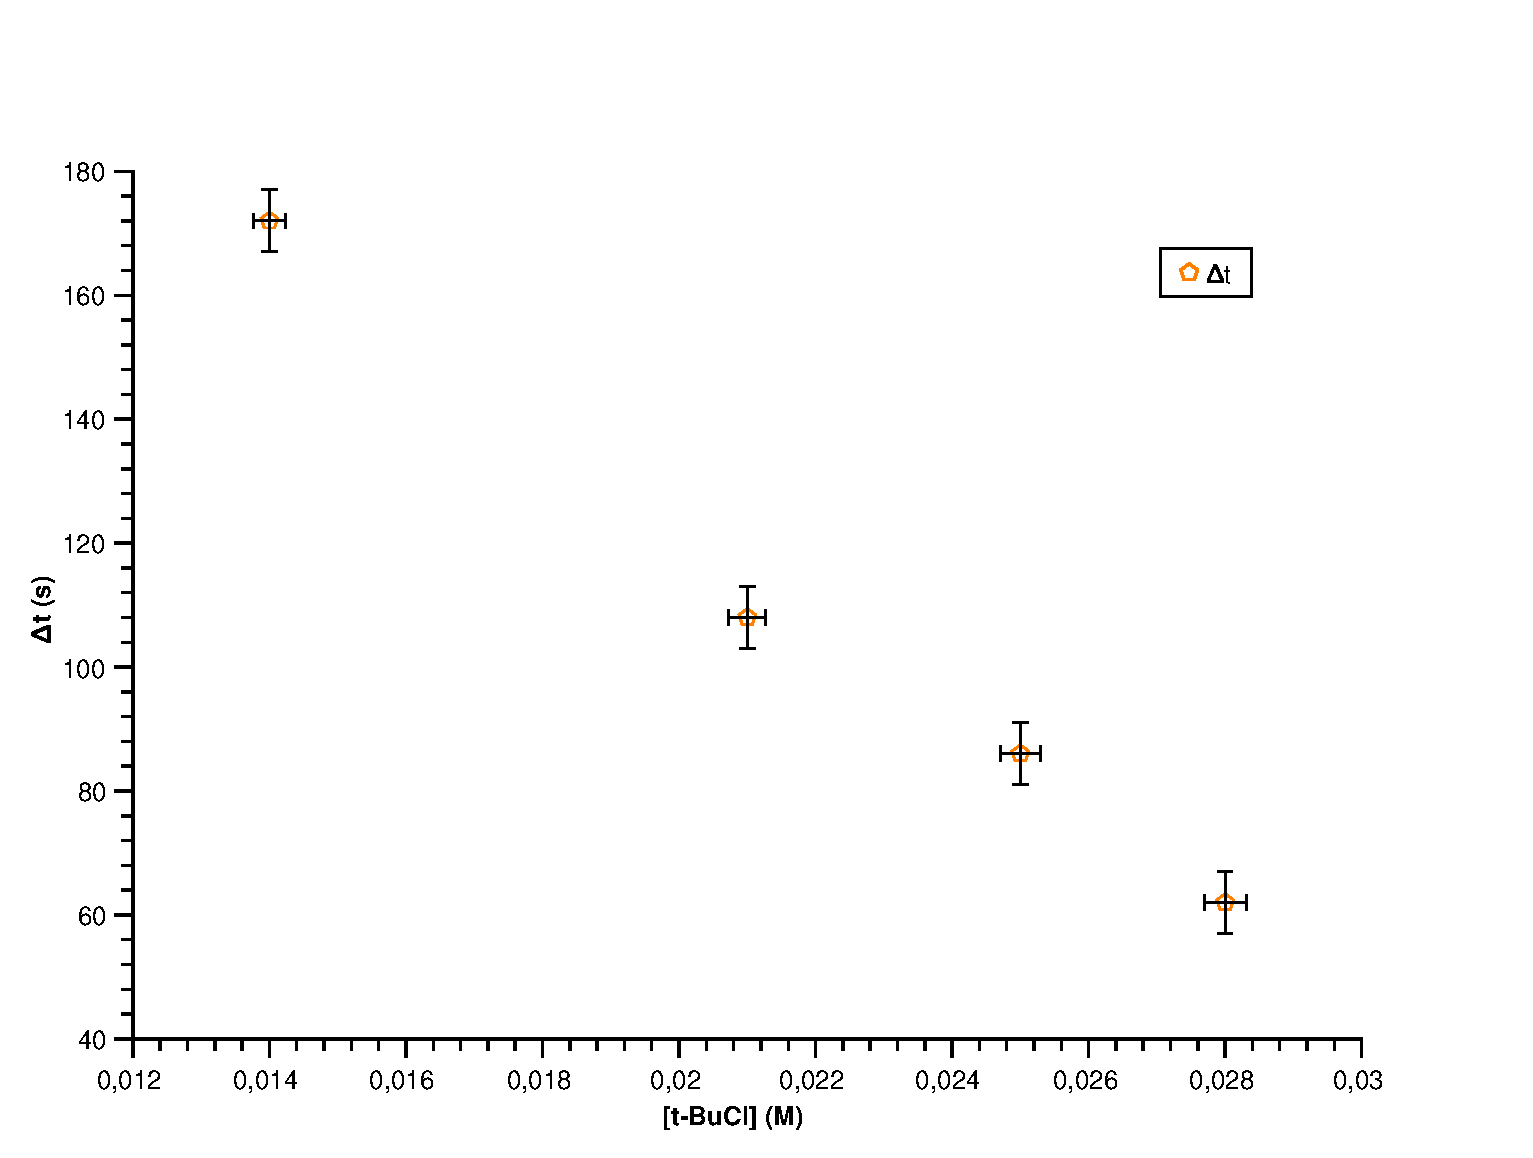
\includegraphics{Graph6.eps}}
    \caption{$\Delta$t([t-BuCl])}
    \label{fig:dt}
\end{figure}
\FloatBarrier

\noindent While the rate of the reaction is usually time dependent, if we assume $n=1$ in equation (\ref{eq:rate}) and that the overall change of the rate is minimal we can use the equation $\nu_0 = \frac{\Delta [\ce{H+Cl-}]}{\Delta t} = \frac{[\ce{NaOH}]}{\Delta t} =k[\ce{(CH3)3CCl}]^n$ a curve for the rate is obtained (see figure (\ref{fig:nu0})). Note that [\ce{NaOH}] is obtained with the dilution formula: 

\begin{align} 
    &C_{initial}V_{initial}=C_{final}V_{final} \Leftrightarrow C_{final} = \frac{C_{initial}V_{initial}}{V_{final}} \nonumber \\ 
    \Rightarrow \ &C_{final,\ NaOH} = \frac{3.0 \ \text{mL} \ \cdot 0.6 \cdot 10^{-2} \ \text{M}}{26 \ \text{mL}} \nonumber \\
    \Rightarrow \ &C_{final,\ NaOH} \approx 6.9 \cdot 10^{-4} \ \text{M} \nonumber \\
    \Rightarrow \  &\boxed{C_{final, NaOH} = (6.9 \pm 0.1) \cdot 10^{-4} \ \text{M}} \nonumber
\end{align}


\begin{figure}[!ht]
    \centering
    \resizebox{0.7\textwidth}{!}{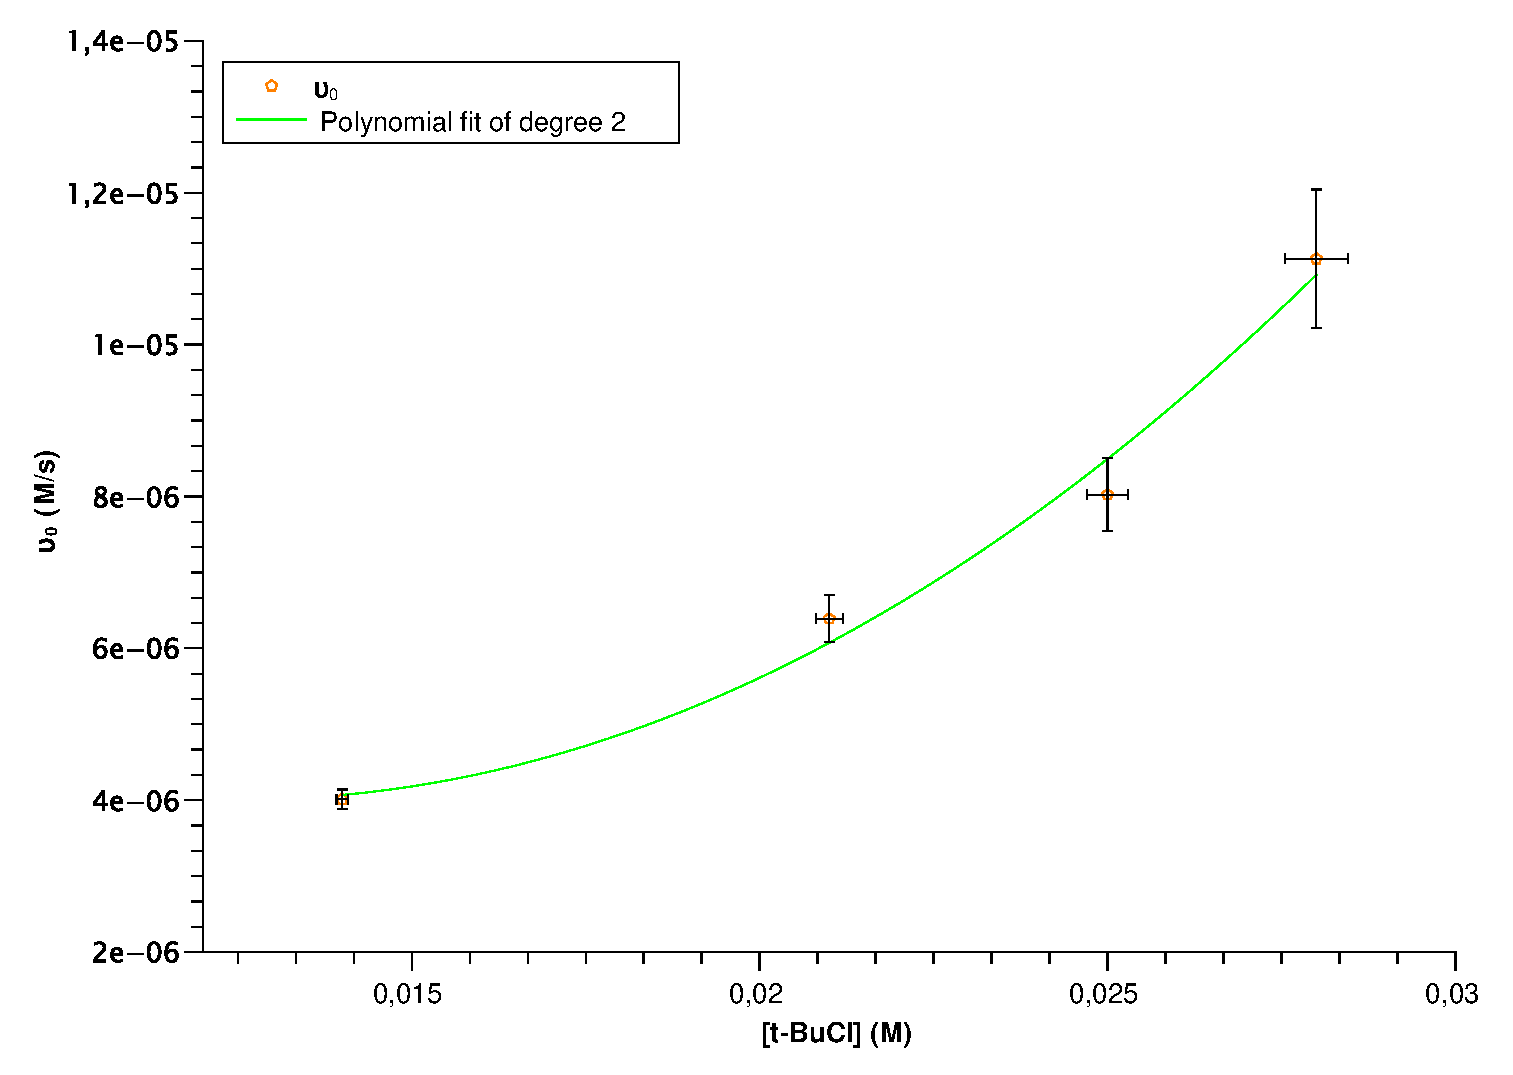
\includegraphics{Graph5.eps}}
    \caption{$\nu_0$([t-BuCl])}
    \label{fig:nu0}
\end{figure}
\FloatBarrier

\noindent The equation for the fit is given by: $\nu_0(x) = a_0 + a_1x +a_2x^2$, with the coefficients in table~(\ref{tab:CoeffsFit})
\begin{table}[!ht]
    \centering
    \begin{tabular}{c|c|c}
        Coefficient & Value & Error \\ \hline
        $a_0$ &  5.9823447962532 $\cdot 10^{-6}$ & 4.3873592363110 $\cdot 10^{-6}$ \\
        $a_1$ & -4.4673588566250 $\cdot 10^{-4}$ & 4.8562004573745 $\cdot 10^{-4}$ \\   
        $a_2$ &  2.1877769219315 $\cdot 10^{-2}$ & 1.2549463091055 $\cdot 10^{-2}$ 
    \end{tabular}
    \caption{Coefficients of the fit}
    \label{tab:CoeffsFit}
\end{table}

\noindent Interestingly, while we get a linear relationship between $\Delta t$ and [t-BuCl] (figure (\ref{fig:dt})), the resulting graph for the rate $\nu_0$ (figure (\ref{fig:nu0})) is not really linear. While trying to fit polynomials of varying degrees, with instrumental weighting, the one with degree 2 had the smallest error. Since $a_2 \gg a_1 \gg a_0$ we conclude \[ \nu_0(x) \approx a_2 x^2 \approx 2.2 \cdot 10^{-2} x^2\] When comparing this equation with equation (\ref{eq:rate}), we deduce \[\boxed{k \approx (2.2 \pm 1.3) \cdot 10^{-2}} \ \text{and} \ \boxed{n \approx 2}\] Contrary to the inital assumption, the collected data implies $n \neq 1$, although there is a lot of room for error. This might question the validity of the experiment, as the calculations of $\nu_0$ have been made on the assumption of $n=1$. To further consolidate this result, we can make a log plot of the date as seen in figure~(\ref{fig:logPlot})

\begin{figure}[!ht]
    \centering
    \resizebox{0.7\textwidth}{!}{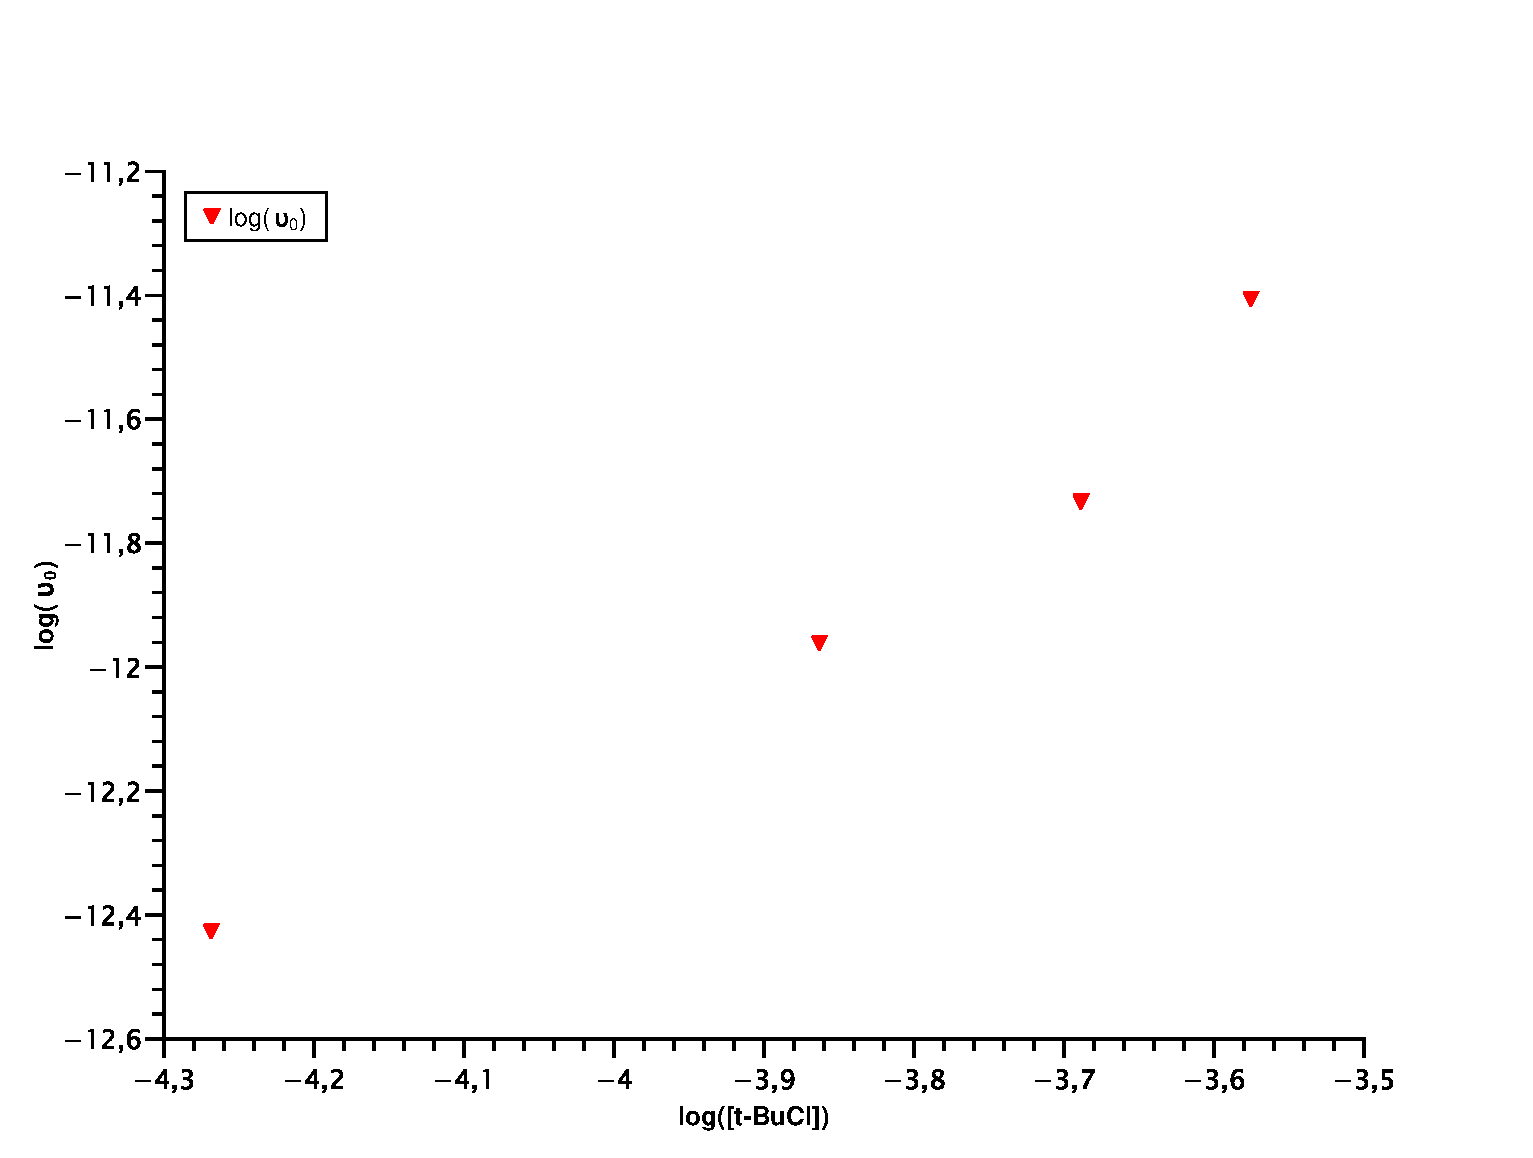
\includegraphics{logPlot.eps}}
    \caption{Plot of log($\nu_0$) as a function of log([t-BuCl])}
    \label{fig:logPlot}
\end{figure}
\FloatBarrier

\noindent As expected, the curve is growing, however neither a slope fit nor a linear fit approximates the data sufficiently good. This implies again that $n \neq 1$.

\subsection{Measurement of the reaction speed at 0°C}
Because of the defective solution of t-BuCl, there was no time to realize this part of the experiment. Nevertheless, we can still use the data from Marie, Maja, Florence and Laura, as seen in table~(\ref{tab:dt0C}).

\begin{table}[!ht]
    \centering
    \begin{tabular}{c|c|c}
        Operator & Temperature($^{\circ}$C) & Elapsed time \\ \hline
        Florence & 1 $\pm$ 0.5   & 29'14'' $\pm$ 5'' \\
        Maja     & 1 $\pm$ 0.5   & 32'18'' $\pm$ 5'' \\
        Marie    & 6.5 $\pm$ 2.5 & 22'21'' $\pm$ 5'' \\
        Laura    & 1 $\pm$ 0.5   & 26'00'' $\pm$ 5''
    \end{tabular}
    \caption{Reaction times of solution 4 at low temperatures}
    \label{tab:dt0C}
\end{table}

\noindent It is a noticeable trend, that the reaction takes significantly longer to finish than at room temperature, about 25' more. Note that an uncertainty was not provided by Laura, Florence and Maja and has therefore been estimated to be 0.5 °C. Similarly, 5'' were added as uncertainty on the time measurement.

\noindent The Arrhenius equation \begin{equation}
    k = Ae^{\frac{-E_a}{k_B T}} 
    \label{arrhenius}
\end{equation} gives us a relationship for k in dependence of temperature. We can also use it to determine the activation energy $E_a$. Note that $A$ is a constant and $k_B$ is the Boltzmann constant. We can rearrange this equation into \cite{arrhenius}: \begin{equation}
    ln(k) = \frac{-E_a}{k_B} \frac{1}{T} + ln(A)
    \label{arrheniusRewrite}
\end{equation} This gives us a linear relationship, which we can use our data with to determine the constants of the equation: the activation energy $E_a$ and the unitless constant $A$. To determine $k$ at 0°C, we use the relation: \begin{equation}
    k = \frac{[NaOH]}{\Delta t \cdot [t-BuCl]}
\end{equation} If we exclude Marie's data point, we get an average value of $\overline{\Delta t} = 29'11''$. We then obtain the average value $\overline{k} \approx 1.4 \cdot 10^{-5}$. The obtained graph is presented in figure~(\ref{fig:arrhenius}).

\begin{figure}[!ht]
    \centering
    \resizebox{0.7\textwidth}{!}{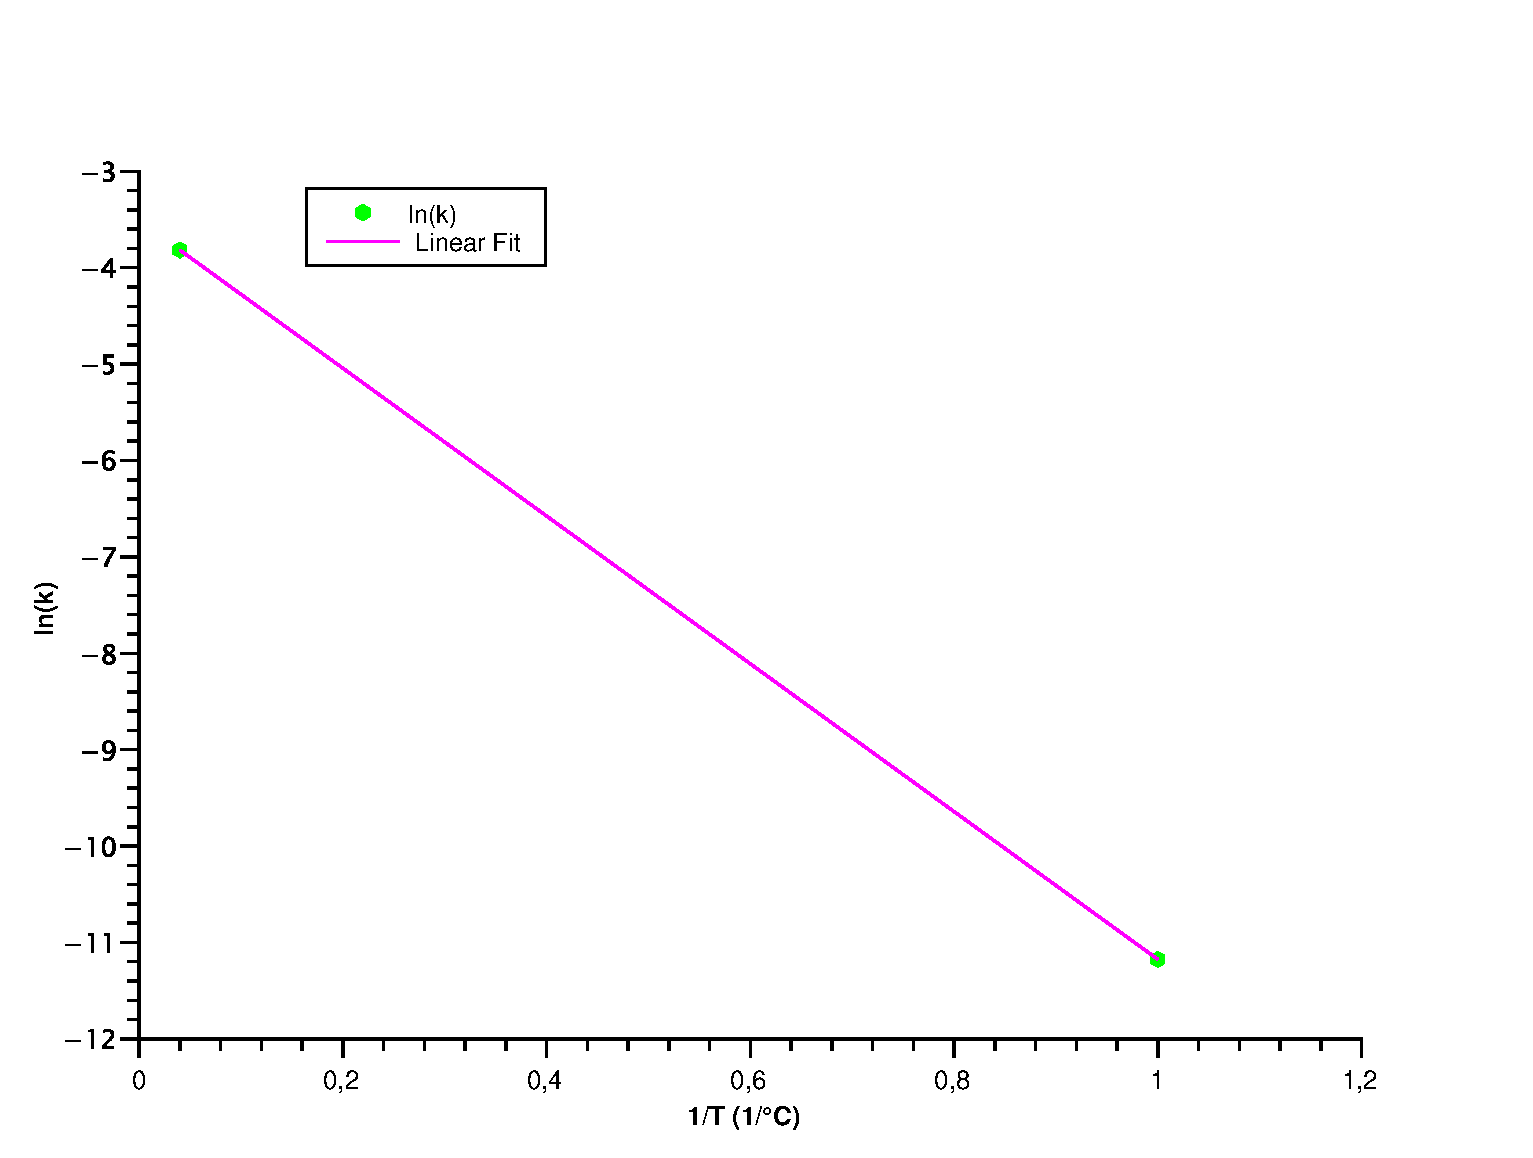
\includegraphics{arrhenius.eps}}
    \caption{Plot of ln(k) as a function of $\frac{1}{T}$}
    \label{fig:arrhenius}
\end{figure}

\noindent The linear fit has equation \begin{equation}
    ln(k) = -7.666396 \frac{1}{T} -3.510057
\end{equation} The slopes gives $\frac{-E_a}{k_B}$ and the oordinates intercept gives $ln(A)$. We determine the constants to be:
\[
\begin{cases}
    E_a = k_B \cdot 7.666396 \approx 1.1 \cdot 10^{-22} \ \text{J} \\
    A = e^{-3.510057} \approx 3.0 \cdot 10^{-2}
\end{cases}
\]

\begin{equation}
    \frac{\partial f(x)}{\partial x} = \iint_\mathbb{R^2} 2x^2\ln(y) dxdy
\end{equation}

\noindent Note that due to the nature of the experiment and the lack of experimental data, the error on these values is very high. It has therefore been omitted to calculate the error, since there is no real value in using only two data points, and the calculated constants should only be seen as a rough estimate of the real values.

\section{Conclusion}
The solvolysis reaction of t-Butyl chloride in water has been found to be dependent on its concentration by the formula $\nu_0 = k \cdot [t-BuCl]^n$, where the constants have been experimentally determined to be (at room temperature): \[ k \approx (2.2 \pm 1.3) \cdot 10^{-2} \ \text{and} \ n \approx 2\] Furthermore, the activation energy of the reaction has been found using the Arrhenius equation to be: \[ E_a \approx 1.1 \cdot 10^{-22} \text{J}\] This experiment has several points in which it can be improved. Firstly, in order to verify that it is actually working, a smarter way to do the experiments would be to start with the quickest one. We lost a lot of time by just waiting on a reaction which might have not even happened. Secondly, the substances used are very volatile, and need to be stored accordingly. During the experiment this was only done half-heartedly with a plastic film above the beakers and should be done with more rigour. Thirdly, the time measurement is one of the most inaccurate. To improve it, a different method than a colour indicator should be used, so that it could be automated with a computer.

\section{Appendix A - Error Calculation}

The error on the volume of the prepared solutions is given by: \begin{align} \Delta V_{total} &= \Delta V_{NaOH} + \Delta V_{\ce{H2O}} + \Delta V_{acetone} + \Delta V_{t-BuCl} \nonumber \\ &= 0.03\ \text{mL} + 0.05\ \text{mL} + 0.1\ \text{mL} + 0.03\ \text{mL} \nonumber \\ &= 0.21\ \text{mL} \nonumber \end{align}

\noindent The error on the concentration of NaOH is then given by: \[ \Delta C_{NaOH} = C_{NaOH} \sqrt{\left(\frac{\Delta V_{NaOH}}{V_{NaOH}} \right)^2+\left(\frac{\Delta V_{total}}{V_{total}} \right)^2} \]

\noindent The error on the concentration of t-BuCl is then given by: \[ \Delta C_{t-BuCl} = C_{t-BuCl} \sqrt{\left(\frac{\Delta V_{t-BuCl}}{V_{t-BuCl}} \right)^2+\left(\frac{\Delta V_{total}}{V_{total}} \right)^2} \]

\noindent The error on the reaction rate $\nu_0$ is given by: \[ \Delta \nu_0 = \nu_0 \sqrt{\left(\frac{\Delta C_{NaOH}}{C_{NaOH}} \right)^2+\left(\frac{\Delta \Delta t}{\Delta t} \right)^2}\]

\begin{thebibliography}{}
    \bibitem{Acetone} \textit{Acetone}, Wikipedia, https://en.wikipedia.org/wiki/Acetone, consulted 26/03/22
    \bibitem{Bromothymol} \textit{Bromothymol blue}, Wikipedia, https://en.wikipedia.org/wiki/Bromothymol$\_$blue, consulted 26/03/22
    \bibitem{T-Butyl Chloride} \textit{tert-Butyl chloride}, Wikipedia, https://en.wikipedia.org/wiki/Tert-Butyl$\_$chloride, consulted 26/03/22
    \bibitem{arrhenius} \textit{Arrhenius equation}, Wikipedia, https://en.wikipedia.org/wiki/Arrhenius\_equation, consulted 02/04/22
\end{thebibliography}

\end{document}
